\documentclass[]{article}
\usepackage{lmodern}
\usepackage{amssymb,amsmath}
\usepackage{ifxetex,ifluatex}
\usepackage{fixltx2e} % provides \textsubscript
\ifnum 0\ifxetex 1\fi\ifluatex 1\fi=0 % if pdftex
  \usepackage[T1]{fontenc}
  \usepackage[utf8]{inputenc}
\else % if luatex or xelatex
  \ifxetex
    \usepackage{mathspec}
  \else
    \usepackage{fontspec}
  \fi
  \defaultfontfeatures{Ligatures=TeX,Scale=MatchLowercase}
\fi
% use upquote if available, for straight quotes in verbatim environments
\IfFileExists{upquote.sty}{\usepackage{upquote}}{}
% use microtype if available
\IfFileExists{microtype.sty}{%
\usepackage{microtype}
\UseMicrotypeSet[protrusion]{basicmath} % disable protrusion for tt fonts
}{}
\usepackage[margin=1in]{geometry}
\usepackage{hyperref}
\hypersetup{unicode=true,
            pdftitle={TMA4285 Timeseries, Exercise 3},
            pdfauthor={Marius Dioli, Amir Ahmed and Andreas Ferstad},
            pdfborder={0 0 0},
            breaklinks=true}
\urlstyle{same}  % don't use monospace font for urls
\usepackage{graphicx,grffile}
\makeatletter
\def\maxwidth{\ifdim\Gin@nat@width>\linewidth\linewidth\else\Gin@nat@width\fi}
\def\maxheight{\ifdim\Gin@nat@height>\textheight\textheight\else\Gin@nat@height\fi}
\makeatother
% Scale images if necessary, so that they will not overflow the page
% margins by default, and it is still possible to overwrite the defaults
% using explicit options in \includegraphics[width, height, ...]{}
\setkeys{Gin}{width=\maxwidth,height=\maxheight,keepaspectratio}
\IfFileExists{parskip.sty}{%
\usepackage{parskip}
}{% else
\setlength{\parindent}{0pt}
\setlength{\parskip}{6pt plus 2pt minus 1pt}
}
\setlength{\emergencystretch}{3em}  % prevent overfull lines
\providecommand{\tightlist}{%
  \setlength{\itemsep}{0pt}\setlength{\parskip}{0pt}}
\setcounter{secnumdepth}{0}
% Redefines (sub)paragraphs to behave more like sections
\ifx\paragraph\undefined\else
\let\oldparagraph\paragraph
\renewcommand{\paragraph}[1]{\oldparagraph{#1}\mbox{}}
\fi
\ifx\subparagraph\undefined\else
\let\oldsubparagraph\subparagraph
\renewcommand{\subparagraph}[1]{\oldsubparagraph{#1}\mbox{}}
\fi

%%% Use protect on footnotes to avoid problems with footnotes in titles
\let\rmarkdownfootnote\footnote%
\def\footnote{\protect\rmarkdownfootnote}

%%% Change title format to be more compact
\usepackage{titling}

% Create subtitle command for use in maketitle
\providecommand{\subtitle}[1]{
  \posttitle{
    \begin{center}\large#1\end{center}
    }
}

\setlength{\droptitle}{-2em}

  \title{TMA4285 Timeseries, Exercise 3}
    \pretitle{\vspace{\droptitle}\centering\huge}
  \posttitle{\par}
    \author{Marius Dioli, Amir Ahmed and Andreas Ferstad}
    \preauthor{\centering\large\emph}
  \postauthor{\par}
      \predate{\centering\large\emph}
  \postdate{\par}
    \date{September 2019}

\usepackage{float} \usepackage[utf8]{inputenc}

\begin{document}
\maketitle

\hypertarget{abstract}{%
\section{Abstract}\label{abstract}}

This article presents the basics of time series analysis, and applies it
to model monthly average atmospheric CO2 levels observed at Mauna Loa
Observatory, Hawaii, U.S. As carbon dioxide is a green house

\hypertarget{introduction}{%
\section{Introduction}\label{introduction}}

Carbon dioxide levels have been monitored since 1958 at the Mauna Loa
Observatory, located in the Pacific Ocean on top of Hawaii's biggest
volcano. Co2 is a green-house gas, and as humans burn fossile fuels,
more is added to the atmosphere. As a consequence we have since the
industrial revolution seen an increase in global average temperature. n
the Paris agreement one targeted to stay below a 2C increase, that is
about equivalent to 450ppm in atmospheric CO2. In this article we will
use theory on time series to model Co2 levels measured at the
observatory, with the goal of forecasting future levels, and to predict
when, if development continues as today, we will reach the 450ppm roof.
For analysis, we will focus on flask measurements taken on a monthly
basis as we are interested in predicting the long-term trend.

\hypertarget{theory}{%
\section{Theory}\label{theory}}

We note that large parts of the theory presented here, is based on
Brockwell and Davis.

A timeseries can be considered as a stochastic process, a set of random
variables indexed in accordance to their occurrence relative to the
other measurements. We will organize the finite timeseries we will deal
with into vectors: \(\mathbf{X}= ( X_1, X_2, \dots,X_n)^T\). A
realization of a timeseries is an observation of the the real values of
the time series, and will be denoted as
\(\mathbf{x} = (x_1, x_2, \dots, x_n)^T\)

The covariance function of two elements of \(\mathbf{X}\) is defined as:
\[\gamma_X(r,s)=Cov(X_r, X_s)=E((X_r-E(X_r))(X_s-E(X_s))\] In general
the covariance function tells us how observations correlate to each
other.

A time series is weakly stationary if:

\begin{itemize}
\item
  \(E(X_t)\) is independent of \(t\)
\item
  \(\gamma_X(t+h, t)\) is independent of t at each h value.
\end{itemize}

In a weakly stationary timesries the correlation between two
observations would only be depended the relative time between the
observation of the repsective observations.

The auto correlation function at a selected lag \(h\) is:
\[\rho_X(h)=\dfrac{\gamma_X(h)}{\gamma_X(0)}\] Where lagging a
time-series is shifting it forward by a selected amount of indexes.

The estimator of the autocovariance of a realized time-series, referred
to as the sample co-variance is:
\[\hat{\gamma}(h)=\frac{1}{n}\sum_{t=1}^{n-|h|}(x_{t+|h|}-\bar{x})(x_{t}-\bar{x})\]
For white noise time-series sample autocorrolation
\(\gamma(h)\sim N(0,\frac{1}{n})\) distribution. Under general
assumptions this estimator is for large samples close to unbiased.

The time series we will observe in the data-analysis later, is
classically decomposed in the following manner:
\[X_t = m_t + s_t + Y_t, \quad t=1,\dots,n\] Where \(EY_t = 0\),
\(s_{t+d}=s_t\) and \(\sum_{j=1}^d s_j= 0\).\(m\) is referred to as the
trend of the time-series, and \(s_t\) is the seasonal trend. The noise
\(Y_t\) is often assumed to be identically independently distributed
(iid) white noise:

\[Y_t \sim WN (0,\sigma^2)\] Subtracting the trend estimation, will
yield as timeseries without a trend. A trend can also be eliminated from
a series by differencing: \[\nabla X_t =X_t-X_{t-1}=(1-B)X_t\] This is
referred to as lag-1 difference, where B is the backward shift operator.
\[BX_t = X_{t-1}\] Can difference n-times by:
\[\nabla^n X_t = (1-B)^nX_t\] Some data, as stated earlier, show a
seasonal trend, this can e.g.~be that months of different years
correlate, applying a lag-d difference operator is a way of reducing
such a case to a stationary process, a lag-d operator can be defined as:
\[\nabla_dX_t = X_t-X_{t-d} = (1-B^d)X_t\]

A time series \(\mathbf{X}\) is a linear process if:
\[X_t = \sum_{j=-\infty}^{\infty}\phi _jY_j\] with
\(\sum_{j=-\infty}^{\infty}|\phi _j|<\infty\). Where \(\mathbf{Y}\) is
white noise.

\hypertarget{arma-and-arima}{%
\subsection{ARMA and ARIMA}\label{arma-and-arima}}

This brings us to the ARMA and SARIMA models, the latter which will be a
central part in our analysis. An \(ARMA(p,q)\) model is defined as the
following: \[\phi(B)X_t = \theta(B)Z_t \] where \(Z_t\) is white noise,
iid with variance \(\sigma^2\)

and the SARIMA; \[\phi(B)\Phi(B)X_t = \theta(B)\Theta(B)Z_ t\] More
specifically we have: \[ARMA(p,q):\quad Y_t=(1-B)^dX_t\]
\[SARIMA(p,d,q)\times(P,D,Q)_s:\quad Y_t=(1-B)^d(1-B^s)^DX_t\] Where:
\[\theta(z)=1+\theta_1z+\dots+\theta_ qz^q\]
\[\Theta(z)=1+\Theta_1z+\dots+\Theta_ Qz^Q\]
\[\phi(z)=1-\phi_1z+\dots+\phi_ pz^p\]
\[\Phi(z)=1-\Phi_1z+\dots+\Phi_Pz^P\] Multiplying the polynomials
together, this is equivalent to a \(ARMA(p+sP,q+sQ)\) model, and fitting
it would thus in essence be equivalent to fitting an ARMA model.

\hypertarget{the-innovations-algorithm}{%
\subsection{The innovations algorithm}\label{the-innovations-algorithm}}

To fit the model one can use the innovations algorithim. Suppose
\(\{ X_t\}\) is zero mean, with \(E(X_t)^2<\infty\) for all t and
suppose \[E(X_iX_j)=\kappa(i,j)\] Denote the best linear predictors, and
their mean squared erros as: \[\hat X_n =\left\{
                \begin{array}{ll}
                  0, n=1 \\
                  P_{n-1}X_n, n \geq 2
                \end{array}
              \right.\] \[\upsilon_n = E(X_{n+1}-P_nX_{n+1})^2\] Where
\(P_i\) is the projection onto the space spanned by the \(i\) first
elements of the timeseries in the \(L^2(\Omega)\) hilbert-space with
inner-product: \[<X_i, X_j> = E(X_iX_j)\]

Define the innovations as:

\[U_n=X_n-\hat X_n\]

and let \(\mathbf{U}\) be a vector with the innovations ranging from 1
to n as its elements. As all \(X_n\) are assumed to be the result of
some linear combination of the preceding values there exists a matrix A
such that

\[\mathbf{U}_n=A_n\mathbf{X}_n\]

\[A = \left[\begin{array}{lllll}
1            & 0            & 0            & \dots & 0 \\
a_{11}       & 1            & 0            & \dots & 0 \\
\vdots       & \vdots       & \vdots       & \ddots & \vdots \\
a_{n-1,-n-1} & a_{n-1,-n-2} & a_{n-1,-n-3} & \dots & 1
\end{array}
\right]\]

This matrix is invertible, as it is is unit lower triangular (it has a
non-zero determinant of 1). The inverse will be on the following form:
\[C_n = \left[
\begin{array}{lllll}
1            & 0            & 0            & \dots & 0 \\
\theta_{11}       & 1            & 0            & \dots & 0 \\
\vdots       & \vdots       & \vdots       & \ddots & \vdots \\
\theta_{n-1,-n-1} & \theta_{n-1,-n-2} & \theta_{n-1,-n-3} & \dots & 1
\end{array}
\right]\] \[A_nC_n=C_nA_n=I_n\] This yields:

\[\hat{\mathbf{X}}_n = \mathbf{X}_n-\mathbf{U}_n = C_n\mathbf{U}_n - \mathbf{U}_n=C_n\mathbf{X}_n-C_n\hat{\mathbf{X}}_n-\mathbf{X}_n+\hat{\mathbf{X}}_n=(C_n-I_n)(\mathbf{X}_n-\hat{\mathbf{X}}_n)\]
Define \[\Theta_n = C_n - I_n\]
\[\Rightarrow \hat{\mathbf{X}}_n=\Theta_n(\mathbf{X}_n-\hat{\mathbf{X}_n})\]
Combining this with the fact that:
\[\mathbf{X}_n = C_n(\mathbf{X}_n-\hat{\mathbf{X}_n})\] solving for the
coefficients above can easily done numerically, Brockwell and Davis
suggest calculating recursively yielding the innovation algorithm:
\[\upsilon_0=\kappa(1,1)\]
\[\theta_{n,n-k}=\upsilon_k^{-1}(\kappa(n+1, k+1)-\sum_{j=0}^{k-1}\theta_{k,k-j}\theta\]
\[\upsilon_n = \kappa(n+1, n+1)-\sum_{j=0}^{n-1}\theta_{ n,n-j} ^2\upsilon_j\]
\#\# ARIMA and the innovation algorithm Forecasting ARMA process using
the innovation algorithim. Assume we have an ARMA process with known
(p,q) values. We transform the process into: \[           \left\{
                \begin{array}{ll}
                  W_t = \sigma^{-1}X_t, \quad t=1,\dots,m\\
                  W_t = \sigma^{-1}\phi(B)X_t, \quad t>m
                \end{array}
              \right.
\] \(m=max(p,q)\) The autocovariance can then be found using:
\[\kappa(i,j)=\left\{
                \begin{array}{ll}
                  \sigma^{-2}\gamma_X(i-j), \quad 1\leq i,j \leq m \\
                  \sigma^{-2}(\gamma_x(i-j)-\sum_{i=1}^p\phi_r\gamma_X(r-|i-j|)), \quad min(i,j)\leq m < max(i,j)\leq 2m\\
                  \sum_{r=0}^q\theta_r\theta_{r+|i-j|}, \quad min(i,j)>m,\\
                  0
                \end{array}
              \right.\] Where applying the innovation algorithim to
\(W\) yields: \[
\left\{
                \begin{array}{ll}
                  \hat W_{n+1} = \sum_{j=1}^n\theta_{nj}(W_{n+1-j}-\hat W _{n+1-j}), \quad 1\leq n < m \\
                  \hat W_{n+1} = \sum_{j=1}^q\theta_{nj}(W_{n+1-j}-\hat W_{n+1-j}), \quad n \geq m
                \end{array}
              \right.
\] This enables us to write \(X_t\) as a linear combination of the
\(W_t\)-s vice versa.

We note: \[\hat W_{n+1} = P_nW_{n+1}\] \[\hat X_{n+1} = P_nX_{n+1}\]
Where P is a projection in the hilbert space \(L^2(\Omega)\).

Using this we get \[
\left\{
                \begin{array}{ll}
                  \hat W_{t} = \sigma^{-1}\hat X_t, \quad 1 \leq t \leq m \\
                  \hat W_{t} = \sigma^{-1}(\hat X_t - \phi_1X_{t-1}-\dots-\phi_pX_{t-p}),\quad t > m
                \end{array}
              \right.
\] Combining this we get: \[X_t - \hat X_t = \sigma(W_t-\hat W_t)\]
which in turns yield: \[
\hat X_{n+1} = \left\{
                \begin{array}{ll}
                  \sum_{j=1}^n \theta _{nj}(X_{n+1-j}-\hat X_{n+1-j}), \quad 1 \leq t < m \\
                  \phi_1X_n \dots + \phi_pX_{n+1+p}+\sum_{j=1}^q\theta_{nj}X\quad t \geq m
                \end{array}
              \right.
\]

\hypertarget{model-comparison-finding-values-for-p-and-q}{%
\subsection{Model comparison, finding values for p and
q}\label{model-comparison-finding-values-for-p-and-q}}

Selecting different values for \(p\) and \(q\) would yield different
models. Using AICC and the AIC criterion is one way of selecting among
these. The methods both base themselves on the idea of scoring on the
likelihood of seeing the realized values given the model and then to
punish the complex models more. We prefer simple models as they are less
prone to over-fitting the data. I.e. will mean square error not be able
to pick up upon this, so more complex models will always be favored,
which is why we should use other criteria as AIC or AICC.

\hypertarget{data-analysis}{%
\section{Data Analysis}\label{data-analysis}}

We start by creating simple time series plot to get an overview.

\begin{center}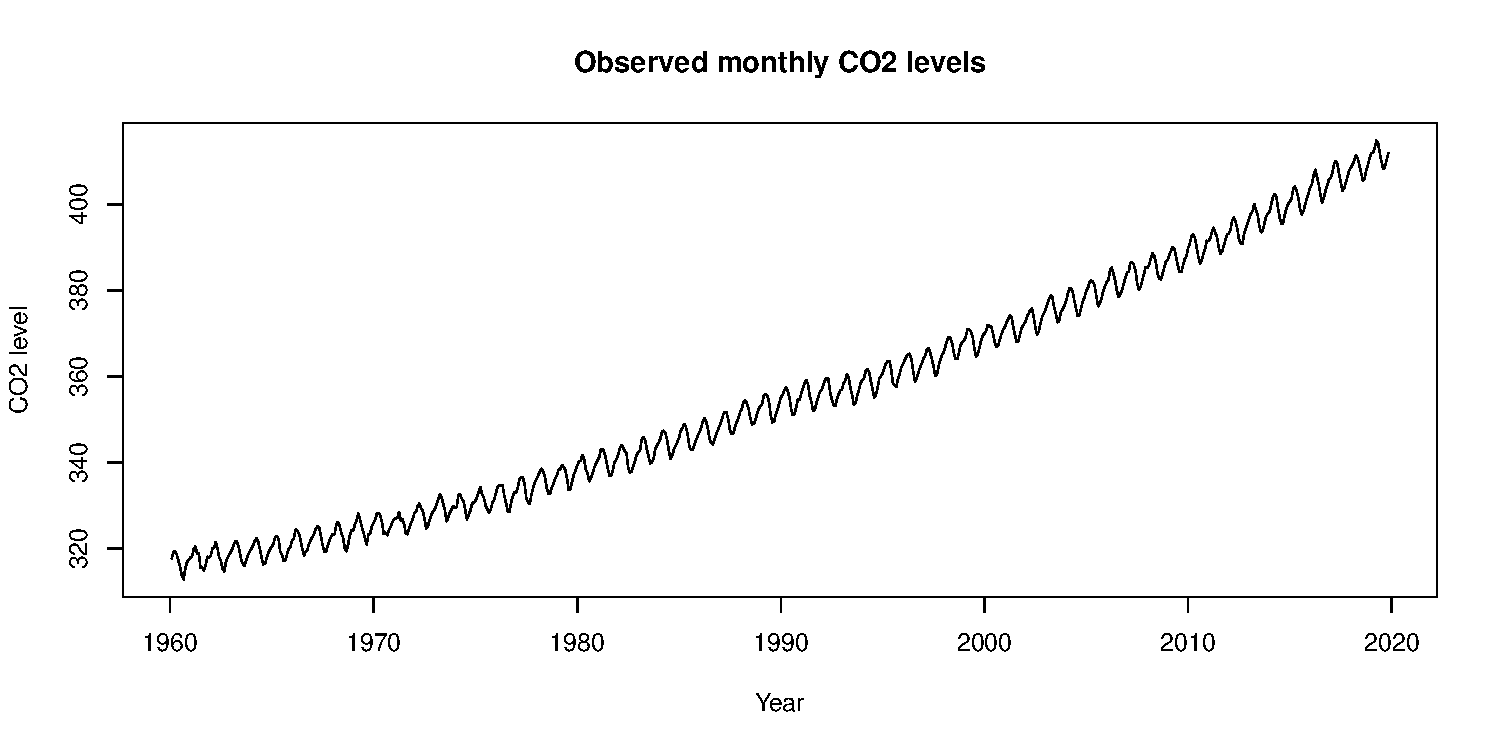
\includegraphics{Tidsrekkerex4_files/figure-latex/unnamed-chunk-3-1} \end{center}

As expected we see an increase. There also seems to be a seasonal trend.

We can decompse the timeseries to get a closer look.

\begin{center}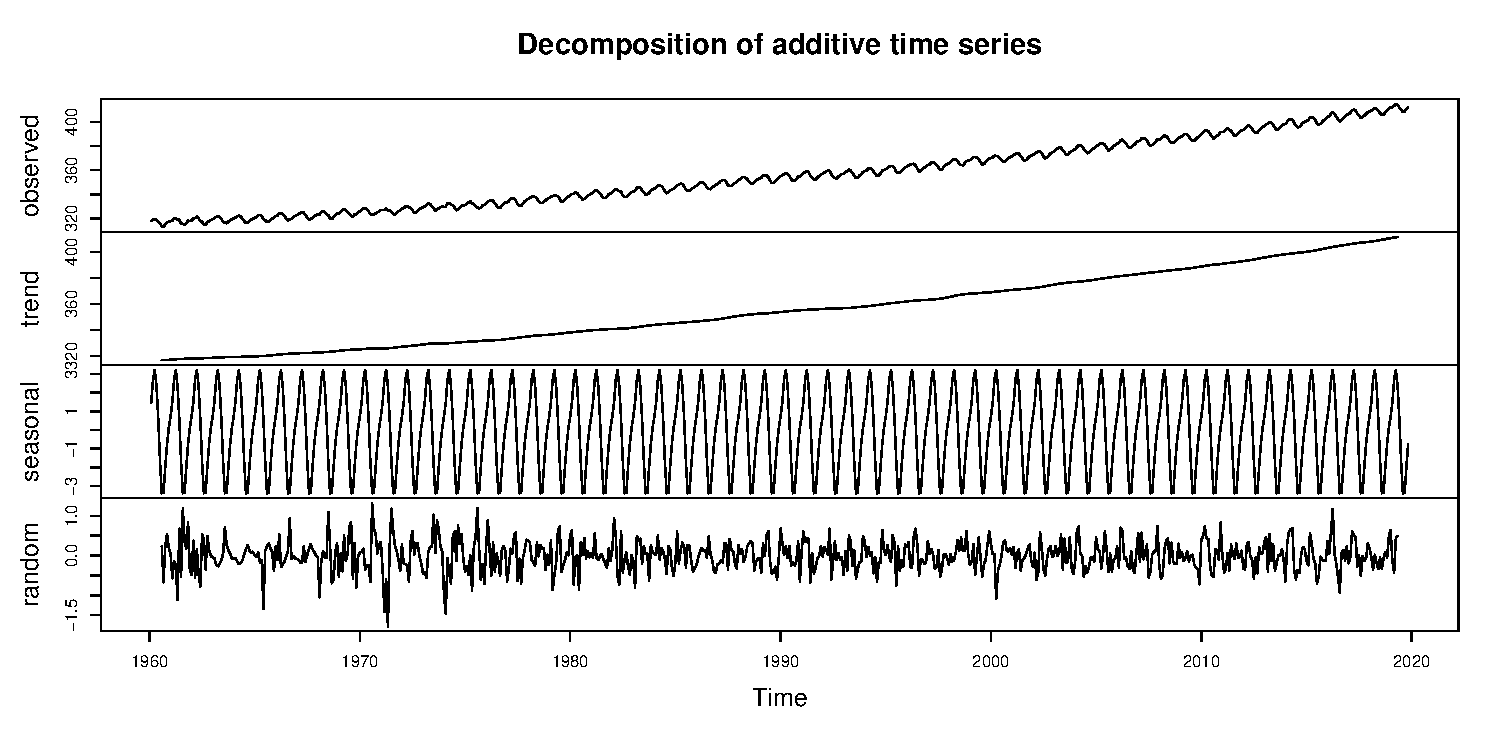
\includegraphics{Tidsrekkerex4_files/figure-latex/unnamed-chunk-4-1} \end{center}

With this we see a much clearer sesonal trend.

We plot the autoccorlation plot for the time series

\begin{center}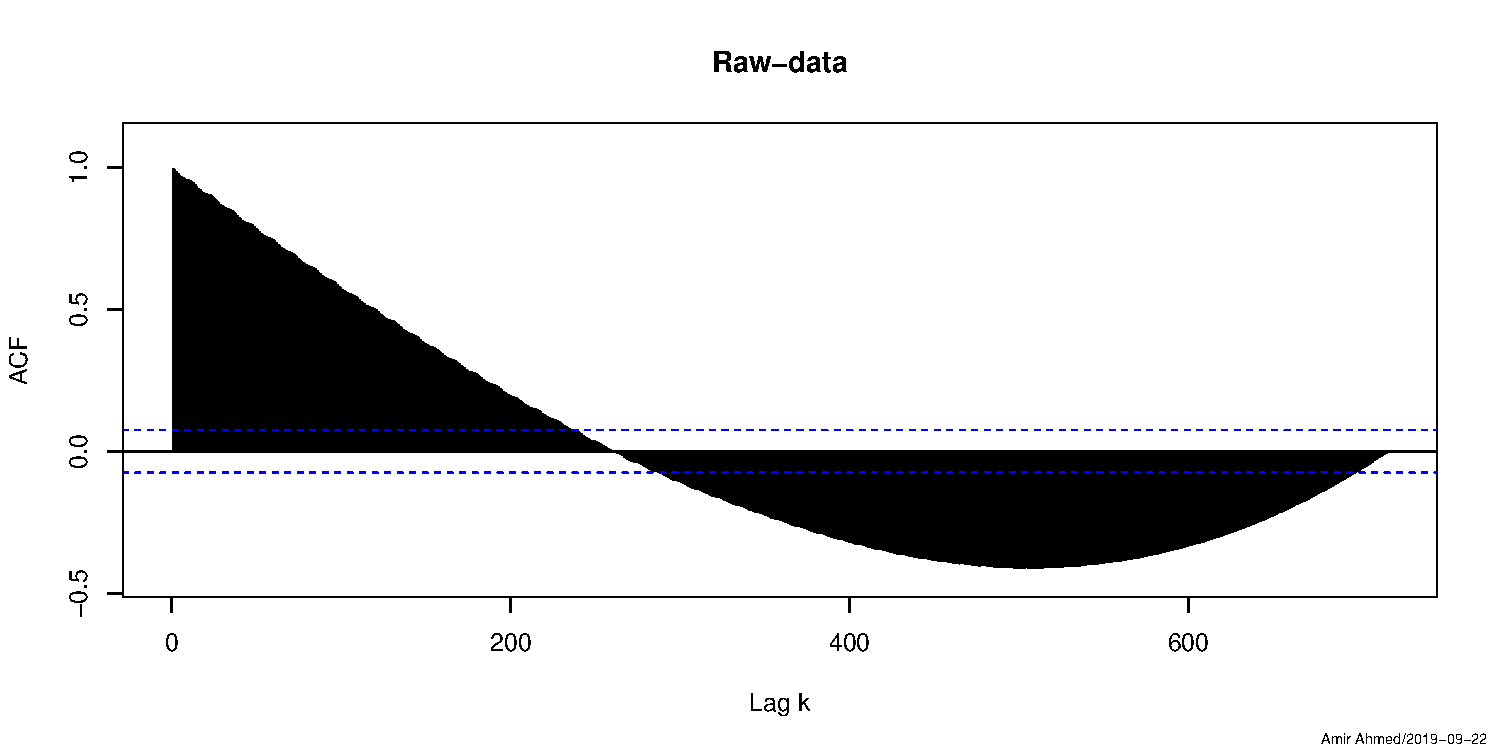
\includegraphics{Tidsrekkerex4_files/figure-latex/unnamed-chunk-5-1} \end{center}

Definitely not stationary, apply differencing (\(\nabla\)) to see if it
gets any better.

\begin{center}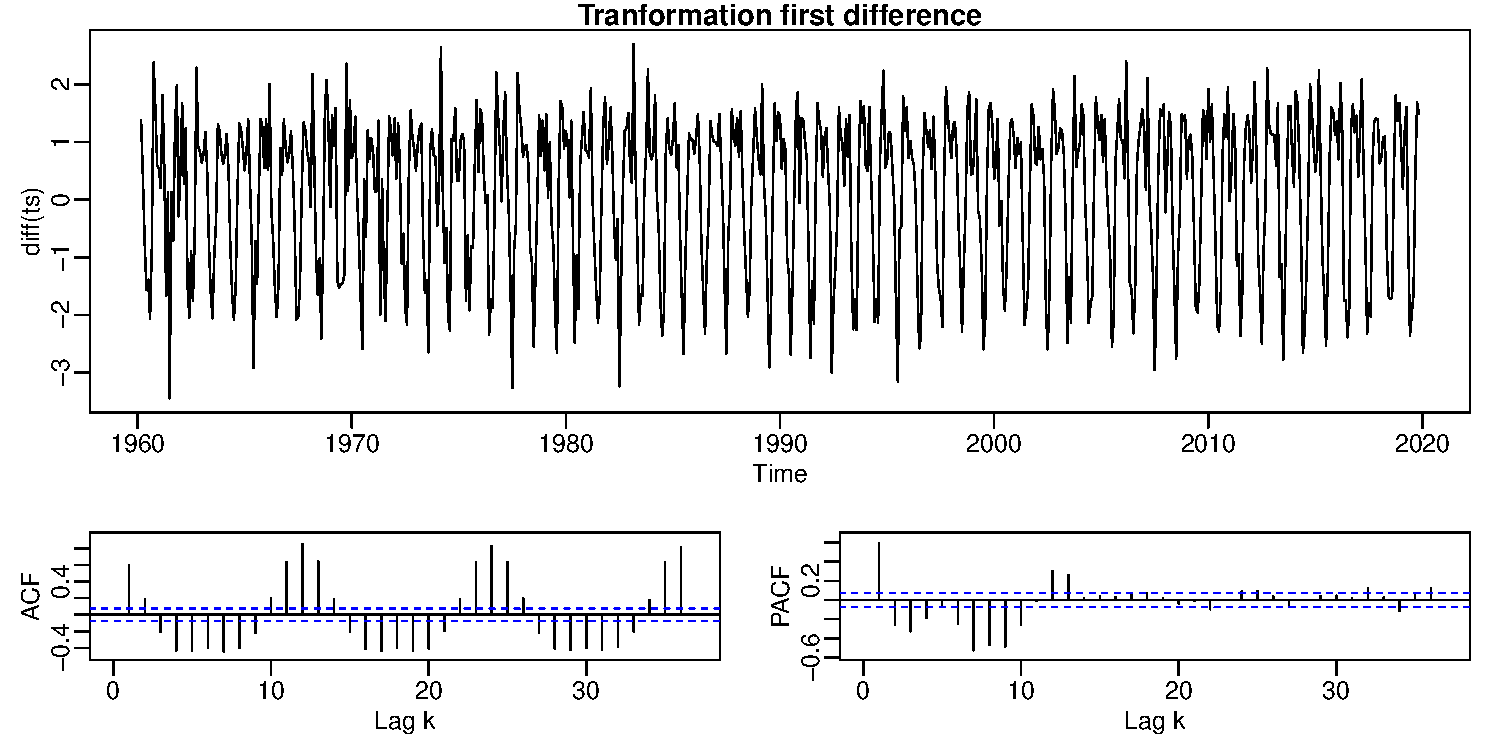
\includegraphics{Tidsrekkerex4_files/figure-latex/unnamed-chunk-6-1} \end{center}

Applying \(\nabla^2\):

\begin{center}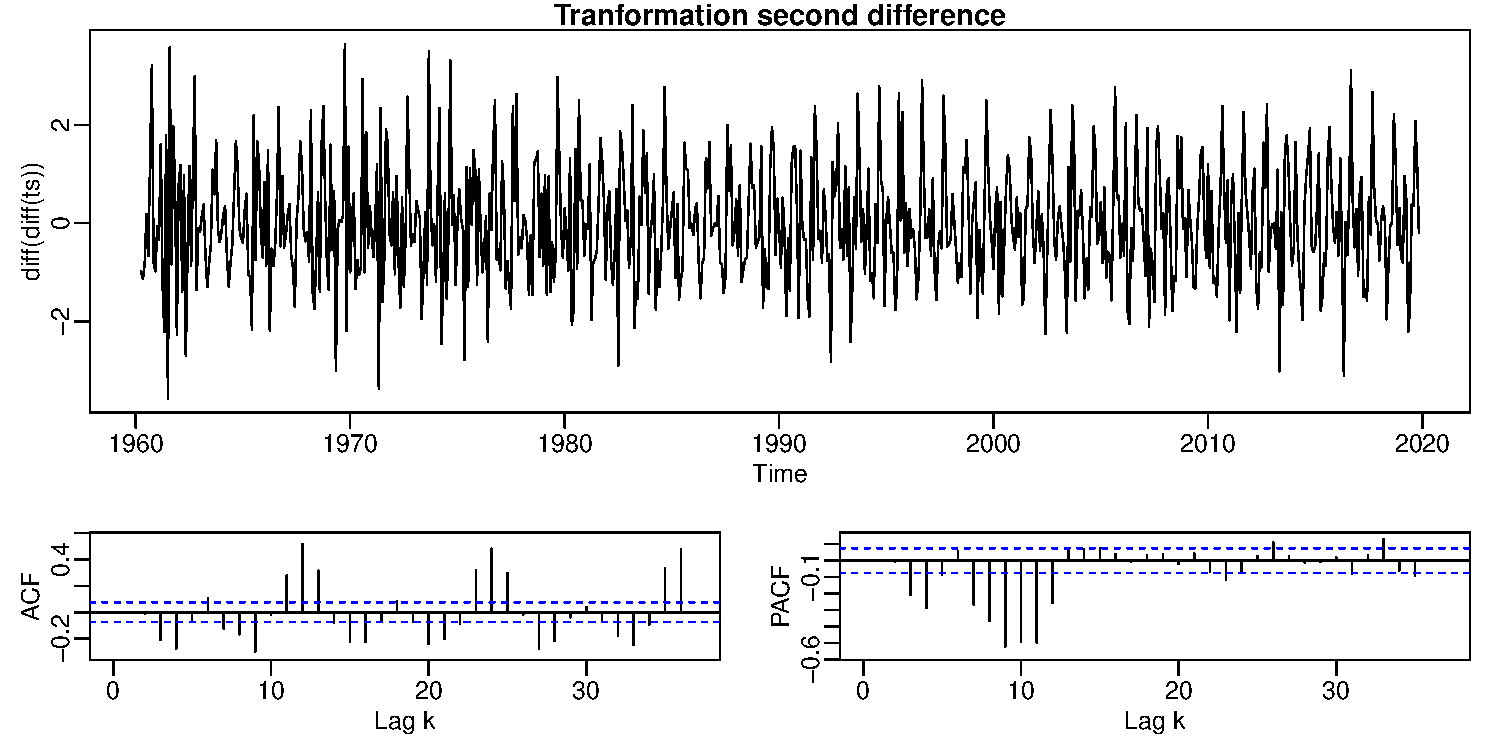
\includegraphics{Tidsrekkerex4_files/figure-latex/unnamed-chunk-7-1} \end{center}

Does not seem to get any better.

We try capturing the seasonal trend. We expect that a season last for a
year, so 12 months seems like a good starting point for differencing.
Applying \(\nabla^{12}\) we get:

\begin{center}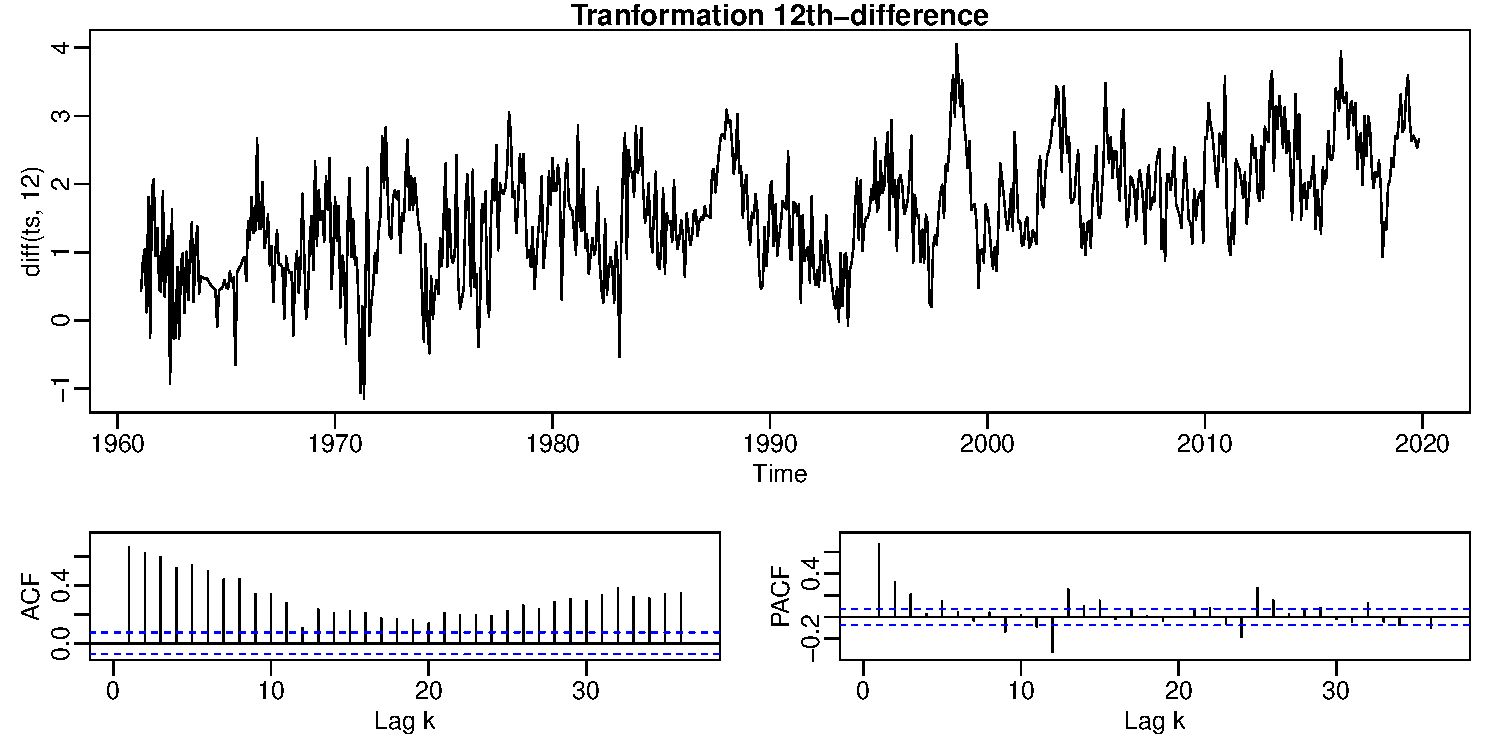
\includegraphics{Tidsrekkerex4_files/figure-latex/unnamed-chunk-8-1} \end{center}

With this it seems we have removed the seasonal component. But it is
clearly not completly stationary. We try applying \(\nabla\nabla^{12}\)
to capture the lag:

\begin{center}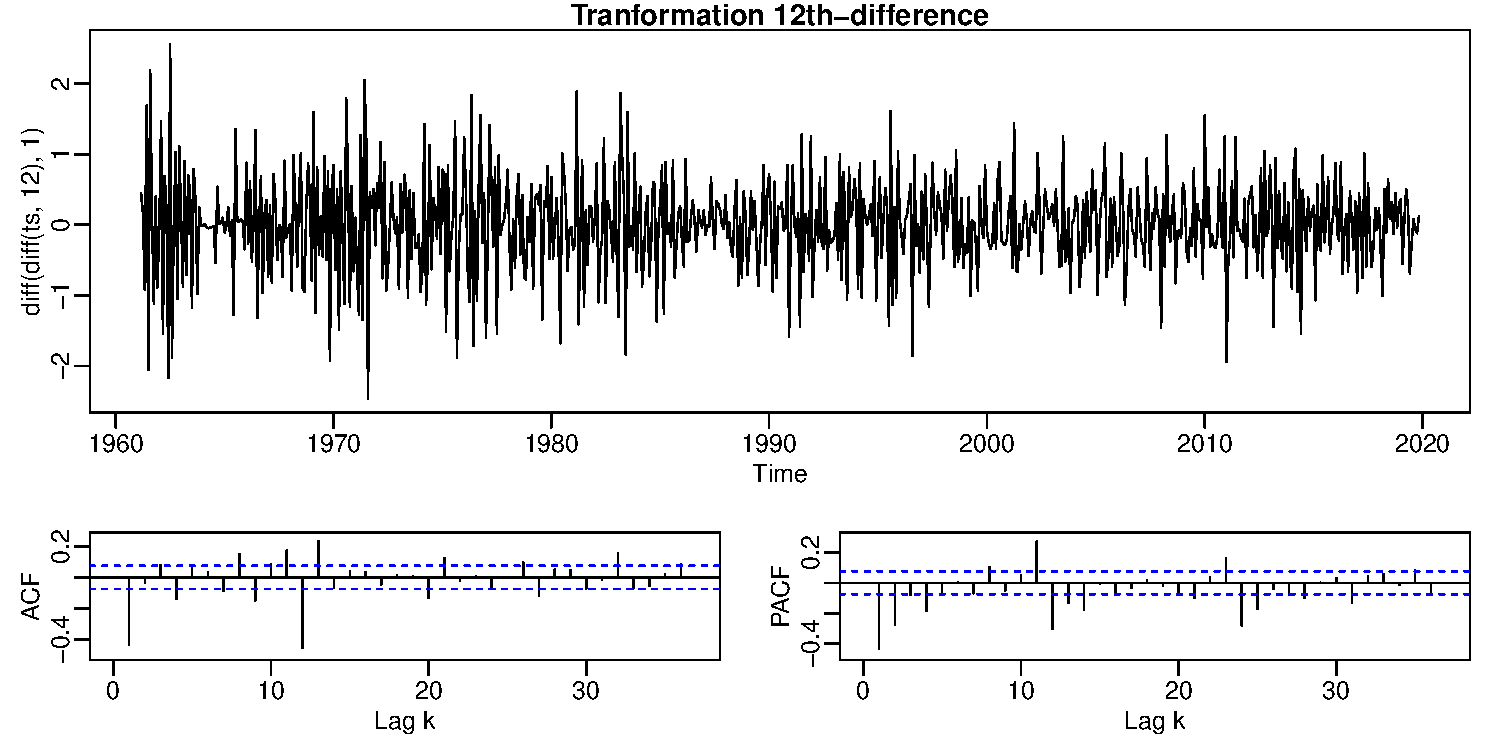
\includegraphics{Tidsrekkerex4_files/figure-latex/unnamed-chunk-9-1} \end{center}

Which seems somewhat stationary, we could increase the lag to get a
better fit, but as we prefer simple models, and we want to avoid
overfitting, we decide to use \(\nabla\nabla^{12}\) to tranform.

We will later see that the acf plot improve form.

There parameters results in a SARIMA model.

(Coefficient can i.e.~be fit using innovations algoritihm. But that
might not be the method impletemented in the package).

To find the best choice of parameters we compare AIC and AICC of
different models.

and \(p=4, d=1, P=5, Q=1\) seems to be best choice of the remaining
parameters, where we get AIC and AICcc values of 1.27

With this chose of parameters our model would be:
\[\phi(B)\Phi(B)X_t = \theta(B)\Theta(B)Z_ t\] \[\theta(z)=1+\theta_1z\]
\[\Theta(z)=1+\Theta_1z\] \[\phi(z)=1-\phi_1z+\dots+\phi_ 4z^4\]
\[\Phi(z)=1-\Phi_1z+\dots+\Phi_5z^5\]

Fitting the model with the selected parameters, we get the following
diagnostic:

\begin{center}\includegraphics{Tidsrekkerex4_files/figure-latex/unnamed-chunk-12-1} \end{center}

\begin{verbatim}
## initial  value -0.393684 
## iter   2 value -0.661896
## iter   3 value -0.765862
## iter   4 value -0.788071
## iter   5 value -0.791576
## iter   6 value -0.792059
## iter   7 value -0.793117
## iter   8 value -0.793789
## iter   9 value -0.794061
## iter  10 value -0.794077
## iter  11 value -0.794083
## iter  12 value -0.794092
## iter  13 value -0.794133
## iter  14 value -0.794148
## iter  15 value -0.794151
## iter  16 value -0.794151
## iter  17 value -0.794151
## iter  17 value -0.794151
## iter  17 value -0.794151
## final  value -0.794151 
## converged
## initial  value -0.787101 
## iter   2 value -0.788459
## iter   3 value -0.790011
## iter   4 value -0.790812
## iter   5 value -0.791655
## iter   6 value -0.791907
## iter   7 value -0.791946
## iter   8 value -0.792014
## iter   9 value -0.792215
## iter  10 value -0.792420
## iter  11 value -0.792517
## iter  12 value -0.792534
## iter  13 value -0.792536
## iter  14 value -0.792536
## iter  15 value -0.792536
## iter  15 value -0.792536
## iter  15 value -0.792536
## final  value -0.792536 
## converged
\end{verbatim}

And the following coefficients:

\begin{verbatim}
##        phi1        phi2        phi3        phi4      theta1        Phi1 
## -0.05851883 -0.06976959 -0.02473830 -0.11904962 -0.51345326 -0.01650475 
##        Phi2        Phi3        Phi4        Phi5      Theta1 
## -0.09926963  0.01414698 -0.11440507 -0.07581437 -0.82967466
\end{verbatim}

The standardized residuals seems to be random, and there are not clear
trend. The residuals seems homoscedastic and are centered at zero, which
is a good indcation that our models assumptions are held by the data.

Looking at the autocorrolation plot, there does not seem to be any lag
corrolating that much. Still, there are a few outliers, but that is
often on 12+ months and can be considered to be well within the range of
some family wise error rate.

Points in the qq-plot also seems to align with the normal line quite
well, which indicate a good fit for our model.

All in all, the model seem to fit the data quite well.

\hypertarget{confidence-interval-for-coefficients}{%
\subsection{Confidence interval for
coefficients}\label{confidence-interval-for-coefficients}}

We use bootstrapping to create confidence intervals for the
coeffiecient. In using bootstraping we create a simulated data-set by
drawing at random from our original data set, and fit a model using
this. We repeat this, and in the end get a set of possible coefficient
values, which we can use to confidence intervals.

For the coefficients we get the following bootstrapped confidence
intervals (95\%) using 200 samples:

\begin{verbatim}
##                  phi1        phi2        phi3       phi4     theta1
## lower 2.5% -0.1822252 -0.28560066 -0.27060160 -0.2218933 -0.7799848
## upper 2.5%  0.4505167 -0.05617251 -0.03621915 -0.0521043 -0.2397842
##                  Phi1        Phi2        Phi3        Phi4        Phi5
## lower 2.5% -0.1527267 -0.17364720 -0.12560727 -0.11921476 -0.10586522
## upper 2.5%  0.0596933  0.05461404  0.07821557  0.05451245  0.04177681
##                Theta1
## lower 2.5% -0.9480253
## upper 2.5% -0.7909041
\end{verbatim}

\hypertarget{forecasting-and-bootstrapping}{%
\subsection{Forecasting and
bootstrapping}\label{forecasting-and-bootstrapping}}

Bootstrapping can also be used to obtain prediction interval. The ones
gained with traditional methods is often too narrow. (REFERENCE) We will
use a a blocked bootstrap, we select adjunct sections the time series at
random and join the selections together.

The method used in this section is adapted from (REFERENCE) chapter on
bootstrapping and bagging.

\begin{verbatim}
## Error in autoplot(ts.bootstrap, colour = TRUE): object 'ts.bootstrap' not found
\end{verbatim}

\begin{verbatim}
## $y
## [1] "Bootstrapped series"
## 
## attr(,"class")
## [1] "labels"
\end{verbatim}

We the fit different models, on 200 bootstrap samples:

\begin{center}\includegraphics{Tidsrekkerex4_files/figure-latex/unnamed-chunk-21-1} \end{center}

\begin{center}\includegraphics{Tidsrekkerex4_files/figure-latex/unnamed-chunk-21-2} \end{center}

\begin{verbatim}
## Error in int_abline(a = a, b = b, h = h, v = v, untf = untf, ...): invalid a=, b= specification
\end{verbatim}

\hypertarget{discussion-and-conclusion}{%
\section{Discussion and Conclusion}\label{discussion-and-conclusion}}

The model seem to predict an increase of the co2 levels in the next few
years, and the data seems to fit the model assumptions. And seem to be
quite confident on its predictions. After

\hypertarget{references}{%
\section{References}\label{references}}


\end{document}
